\begin{exercise}
  Schreiben sie ein Programm, welches das Stabilitätsgebiet
  eines beliebigen, linearen Mehrschrittverfahrens grafisch
  darstellt. Testen Sie mit den Ihnen bekannten impliziten
  und expliziten linearen Mehrschrittverfahren. Insbesondere
  sollen Sie Adams-Bashford Verfahren (Example 5.5),
  Adams-Moulton Verfahren (Example 5.6) und BDF Verfahren
  (Aufgabe 41) verschiedener Ordnung testen.

  Hinweis: Sie können ein Computeralgebrasystem verwenden.
  Alternativ können die Nullstellen eines Polynoms über die
  Eigenwerte der Begleitmatrix numerisch berechnet werden.
\end{exercise}

\begin{solution}
\begin{figure}
    \centering
    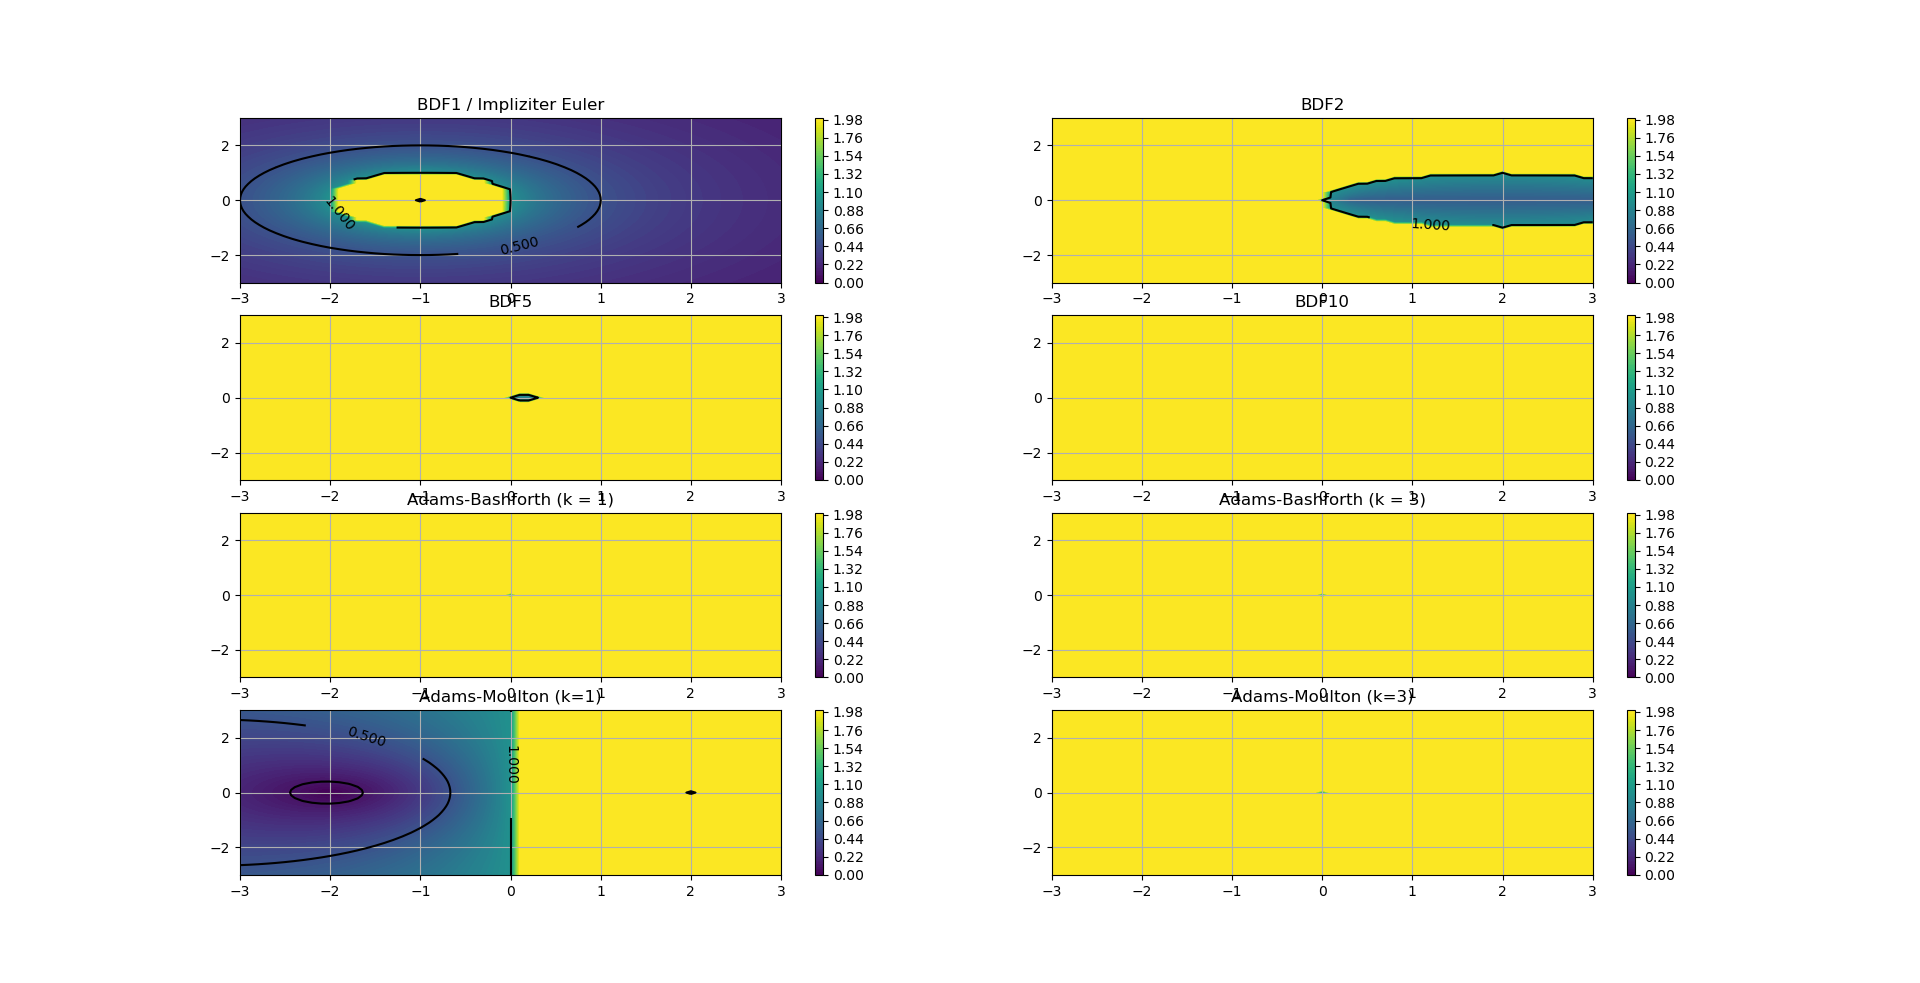
\includegraphics[width=\linewidth]{plot46.png}
\end{figure}
\FloatBarrier
\end{solution}
